\chapter{Il contesto aziendale}
\label{chap:introduzione}
\noindent
\textit{Nel seguente capitolo presento il contesto organizzativo e produttivo dell'azienda Bluewind S.R.L., presso la quale ho svolto la mia attività di tirocinio.
Durante la mia permanenza in azienda ho avuto modo di discutere con diversi colleghi sulla loro realtà lavorativa, e mi sono informato quanto più possibile sul tipo di attività che svolgono.
Questo capitolo contiene le informazioni sull'organizzazione, i metodi di lavoro e la cultura aziendale di Bluewind che sono riuscito ad apprendere durante quest'esperienza.}
\section{\textit{Bluewind}: aree di attività e mercati di riferimento}
\iffalse
\textit{In questa sezione faccio un'introduzione all'azienda \textit{Bluewind} S.R.L., presso la quale ho svolto l'attività di stage.
Descrivo le loro aree di mercato e il tipo di progetti dei quali si occupano.}\\\\
\fi
\noindent
Fondata nel 1998, \textit{Bluewind} è un'azienda informatica specializzata nel campo dei sistemi \textit{embedded} e della sicurezza informatica.
Si occupa sia dello sviluppo di prodotti \textit{software} per aziende nell'ambito industriale, medico e dell'\textit{automotive}, sia di fornire ad altre aziende servizi nell'ambito della sicurezza informatica e della \gls{func_saf_g}.\\\\
\noindent
Dal punto di vista dello sviluppo \textit{software}, gli anni di esperienza nel settore hanno permesso all'azienda di accumulare un bagaglio di conoscenze e competenze che, ad oggi, gli permette di occuparsi dell'intero ciclo di vita di un prodotto.
L'azienda infatti non si occupa solo dell'implementazione del codice ma è coinvolta in tutti gli stadi del progetto:
\begin{itemize}
    \itemsep0em
    \item l'analisi dei requisiti
    \item la scelta e la progettazione dell'\textit{hardware}
    \item la progettazione del \textit{software}
    \item la stesura del codice
    \item lo sviluppo dei test
    \item le verifiche di sicurezza
\end{itemize}
Occorre tuttavia sottolineare che, in base alle richieste e necessità dei clienti, non necessariamente spetta sempre all'azienda occuparsi di ogni singolo passaggio di questo ciclo di vita.\\

\noindent
Un'aspetto molto importante del settore in cui opera \textit{Bluewind} è la presenza, per molti campi di utilizzo dei prodotti \textit{embedded}, di normative e \textit{standard} da rispettare per soddisfare i requisiti di sicurezza di alcuni settori critici.
Per questo motivo \textit{Bluewind} ha raccolto al suo interno una significativa conoscenza sulla \textit{functional safety}, arrivando ad offrire servizi di consulenza e di validazione su questo tema ad aziende terze, e riuscendo a fare di questo ambito uno dei suoi principali punti di forza e competitività.\\
La disciplina della \textit{functional safety} si occupa di garantire che un sistema si comporti in maniera prevedibile e che eventuali errori non portino al rischo di provocare danni.\\
Un caso pratico che si può prendere in esempio, per dimostrarne l'importanza, è quello di un impianto con vari macchinari ed componenti automatizzati e in movimento, all'interno del quale possono essere presenti degli operatori.
In questo caso è fondamentale che il comportamento di tutte le componenti dell'impianto sia prevedibile, e che anche nell'eventualità di un un errore \textit{software}, o guasto \textit{hardware}, non si arrivi a una situazione di rischio che possa provocare dei danni a persone o cose.\\
Questo è quindi un aspetto molto importante, e necessita che i requisiti delle norme e degli \textit{standard} tecnici vengano considerati all'interno del ciclo di vita di un prodotto fin dall'inizio.\\
Per accertare che durante la progettazione e lo sviluppo siano stati seguiti tali vincoli ci si affida a degli enti certificatori, che fanno una revisione della documentazione relativa al progetto e valutano che poi tutto sia coerente.
Recentemente Bluewind ha accolto all'interno del suo \textit{team} alcuni dipendenti che hanno già lavorato in passato come enti certificatori, in modo da poter rafforzare le proprie competenze nella materia.\\

\noindent
Ad oggi, \textit{Bluewind} è presente sul territorio con due sedi: una sede principale, a Castelfranco Veneto (VI), che si occupa delle attività di ricerca, sviluppo e \textit{marketing}, e una sede secondaria a Milano focalizzata sulla \textit{functional safety} e sulla sicurezza informatica in generale.


\section{L'organizzazione aziendale e il metodo di lavoro}
\iffalse
In questa sezione descrivo in che modo i dipendenti dell'azienda vengono suddivisi in gruppi, i loro ruoli, come gestiscono le loro interazioni e la pianificazione del lavoro.
\fi
\subsection{I ruoli}
\noindent
L'azienda è suddivisa in due macro reparti, ognuno dei quali è gestito da un responsabile : il reparto \textit{Sales and Marketing}, incaricato degli aspetti commerciali, pubblicitari, di vendita dei prodotti, e il reparto \gls{ReD} che invece si occupa dell'analisi e sviluppo dei prodotti e della ricerca tecnologica.\\
Durante la mia attività di tirocinio sono stato inserito all'interno del reparto \textit{R\&D} e ho avuto modo di conoscere i principi alla base del loro metodo di lavoro.\\\\
\noindent
All'interno del reparto, i dipendenti ricoprono diversi tipi di ruoli:
\begin{itemize}
	\itemsep0em
	\item \textbf{Analisti} : si occupano di studiare la realtà in cui si colloca il prodotto, analizzare il problema e stendere quali requisiti è necessario che il prodotto soddisfi, affinché possa adempiere al suo compito.
	Siccome la realizzazione di un progetto aziendale coinvolge, inevitabilmente, diverse materie, e ognuna di esse richiede specifiche conoscenze, gli analisti si dividono a loro volta in categorie in base allo specifico settore di competenza:
	\begin{itemize}
	    \itemsep0em
			\item \textbf{Analisti \textit{hardware}} : siccome \textit{Bluewind} fornisce e progetta componenti \textit{hardware} su misura, ha nel suo \textit{team} alcuni membri incaricati di capirne le necessità e valutare l'impatto che può avere il malfunzionamento di alcune componenti.
			\item \textbf{Analisti \textit{software}}
			\item \textbf{Analisti della sicurezza} : si differenziano per la loro conoscenza specifica nei temi della sicurezza informatica, e, nel particolare, delle norme e degli \textit{standard} che ne regolamentano il tema
	\end{itemize}
	\item \textbf{Sviluppatori \textit{software}} : nel caso di \textit{Bluewind} gli sviluppatori non svolgono solo le attività di stesura del codice, ma assumono anche il ruolo di progettisti, collaborando insieme agli analisti e ai clienti per interpretare al meglio i bisogni di quest'ultimi
	\item \textbf{Specialisti di \textit{Functional Safety}} : data la rilevanza del tema della \textit{functional safety}, all'interno dell'azienda vi è un gruppo di addetti che si occupa esclusivamente di questa materia
	\item \textbf{\textit{Product Owner}} : i \gls{po} sono i responsabili del progetto; si occupano di interfacciarsi con il cliente, gestire la parte di \textit{report} delle attività, supervisionare il \textit{team} di sviluppo, arrivando anche a prendere in carico aspetti burocratici e relativi alla fatturazione
	\end{itemize}

	\begin{figure}[H]
    \centering
    \makebox[\textwidth][c]{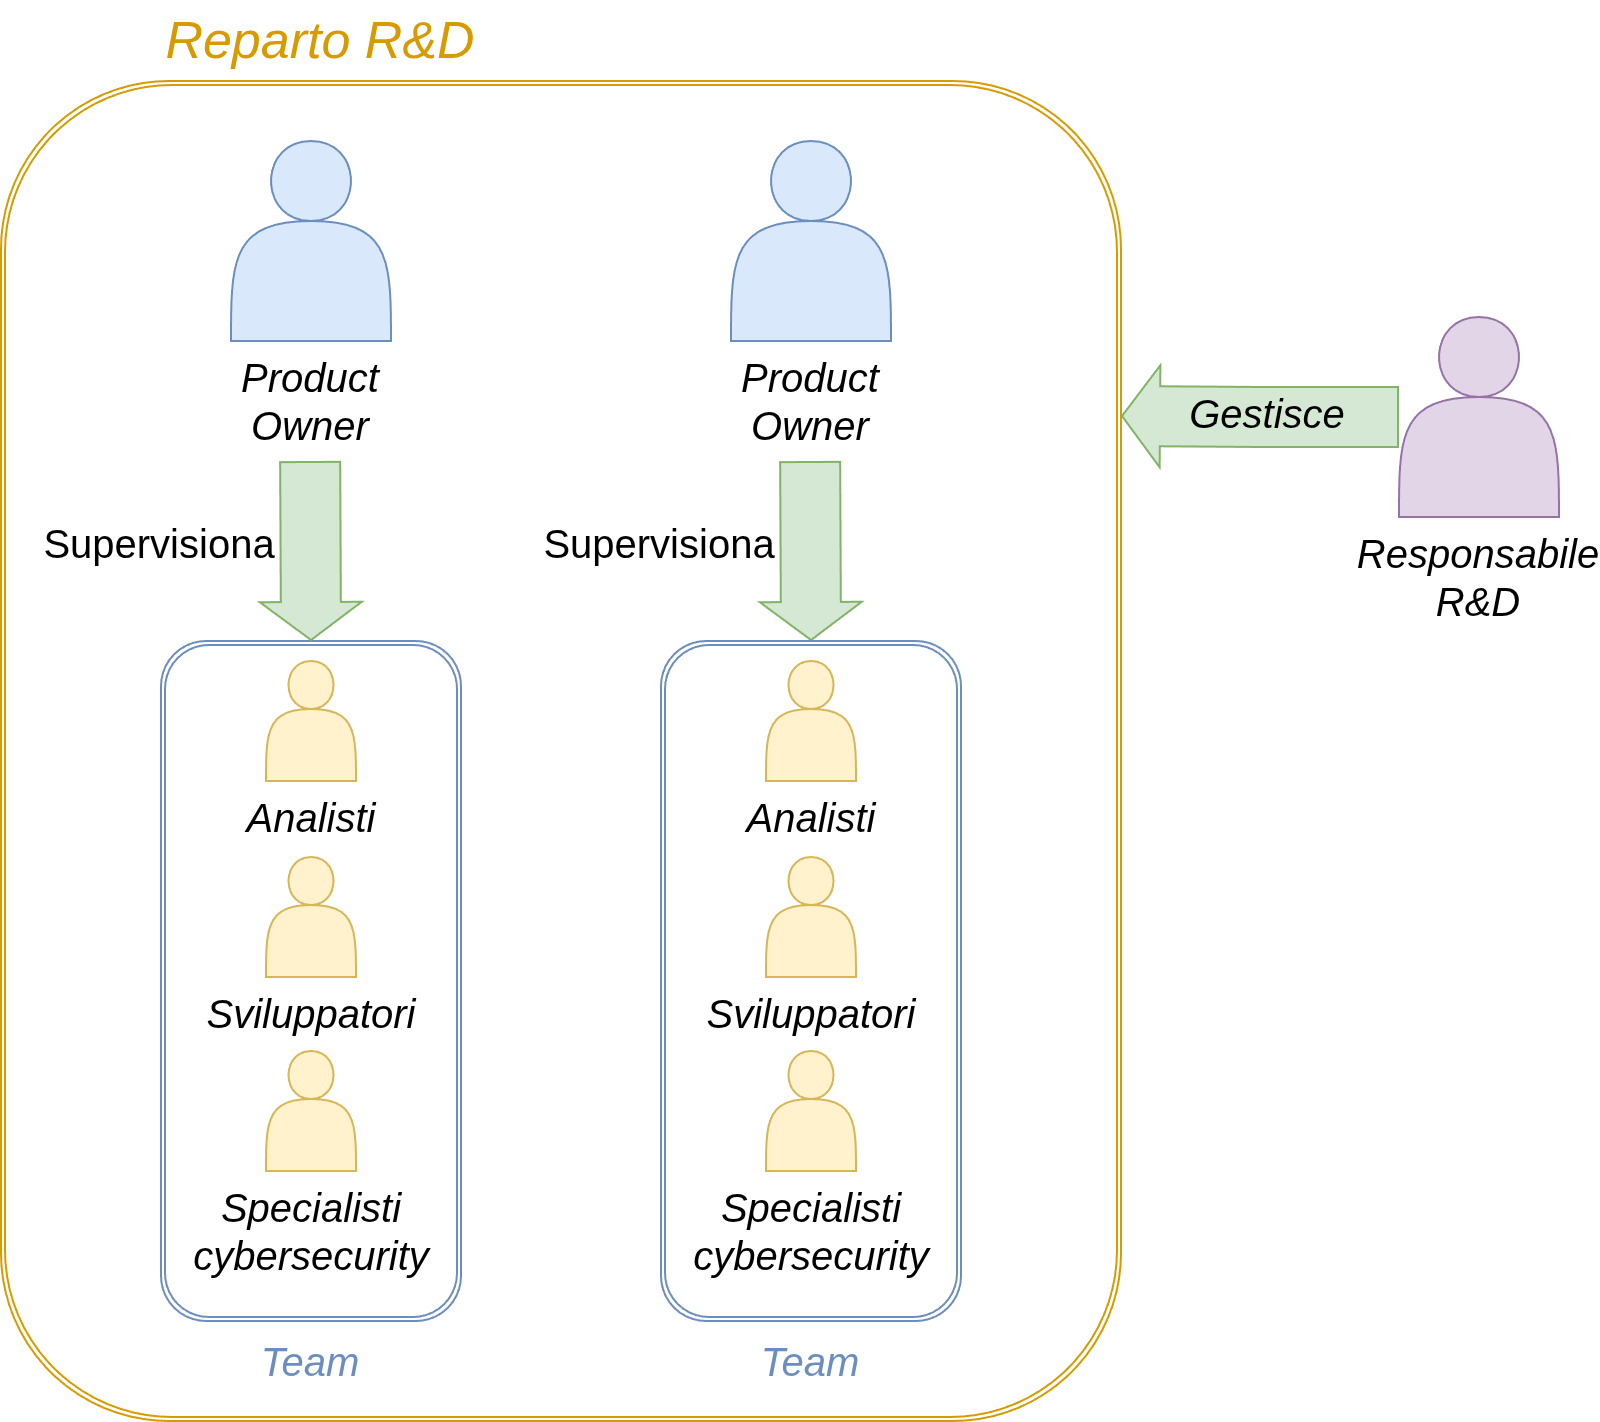
\includegraphics[width=\textwidth]{img/organizzazione_ruoli.png}}
    \caption{\centering Rappresentazione grafica di un esempio di gerarchia dei ruoli all'interno dell'azienda.}
    \vspace{0.1cm}
    {\footnotesize Elaborazione originale dell'autore\par}
	\end{figure}
\subsection{Il metodo \textit{Agile}}
\noindent
All'interno di \textit{Bluewind} ho avuto modo di osservare come l'adozione del metodo \gls{agile_g} non sia una prerogativa dello sviluppo \textit{software}, inteso come il processo specifico di progettazione e implementazione di un prodotto, ma che i suoi principi possano integrarsi efficacemente anche all'interno di processi aziendali più generici e ampi.\\
Da quello che ho potuto cogliere, nell'organizzazione aziendale di \textit{Bluewind} la metodologia \textit{agile} non si limita a regolare il metodo di avanzamento dei progetti e delle attività dell' \textit{R\&D}, ma rappresenta anche un importante fondamento del loro modello economico.\\

\noindent
Per l'organizzazione dei progetti, l'azienda adotta nello specifico il \textit{framework} \gls{scrum_g}, dividendo i progetti in \textit{sprint} di una o due settimane.
I progetti sono assegnati a \textit{team} di circa 3 persone (o più, in base al carico di lavoro), tra sviluppatori e analisti, con alla direzione un \textit{product owner} che volge il ruolo di \textit{scrum master}. Quest'ultimo si occupa quindi di agevolare la corretta applicazione del \textit{framework scrum}.\\
In base alla necessità è possibile che alcuni dipendenti si occupino nello stesso periodo di più progetti in simultanea, tuttavia è una situazione che si cerca di evitare, spingendo su una suddivisione del lavoro più omogenea tra il personale.\\

\noindent
All'inizio della collaborazione, il cliente acquista un determinato numero di \textit{sprint} durante le quali il \textit{team} di \textit{Bluewind} si andrà a occuparsi del progetto.
Agli sviluppatori e agli analisti viene dato l'incarico di definire le attività da svolgere per il proseguimento del progetto, valutando il tempo necessario per ognuna di esse.\\
In mancanza di una richiesta diversa, esplicita del cliente, una \textit{sprint} si protrae per due settimane, con al suo interno diverse riunioni di sincronizzazione che coinvolgono sia il \textit{team} di sviluppo di \textit{Bluewind}, sia i rappresentati della parte cliente.
Non di rado accade che nelle riunioni di aggiornamento a confrontarsi sia il personale tecnico delle due parti.
Questo permette al cliente di avere una visione molto più nel dettaglio di come procedono i lavori ed, eventualmente, di dare un \textit{feedback} molto più diretto su come si preferisce che vengano gestite certe questioni.
Coinvolgere il cliente ai vari stadi del progetto e motivarne la partecipazione, con una frequenza di riunioni che va oltre quella di un approccio \textit{agile} classico, è uno dei principali impegni di \textit{Bluewind}, che ha saputo dimostrare la sua efficacia.\\
Esaurito il numero di \textit{sprint} a disposizione, il cliente può decidere se proseguire con lo sviluppo del progetto acquistandone altre, nel caso desiderasse aggiungere funzionalità o andare ad apportare migliorie.
Nella stessa maniera viene gestito anche un eventuale piano di manutenzione e aggiornamento del prodotto.\\\\
A questo metodo di gestione del lavoro si legano poi anche altri processi aziendali, che non necessariamente sono coinvolti direttamente nell'evoluzione del prodotto, ma hanno la loro significativa rilevanza sia nella visione del progetto come sua intero, sia a livello di organizzazione aziendale.

\section{I clienti}
\iffalse
In questa sezione descrivo il tipo di clientela a cui si interfaccia l'azienda, descrivendo i diversi tipi di relazione azienda-cliente che ci possono essere.
\fi
\noindent
Occupandosi di sistemi \textit{embedded}, i domini applicativi dei prodotti e dei servizi di \textit{Bluewind} spaziano in molteplici mercati.
Tra i suoi clienti una buona maggioranza arriva dai settori dell'\textit{automotive}, dell'automazione industriale, dei sistemi di domotica e dell'elettronica di consumo.\\\\
Il modo con cui vengono mantenuti i rapporti e le interazioni con questi clienti può cambiare in base al loro settore di appartenenza.
Un chiaro esempio è il mondo dell'\textit{automotive}: all'interno dell'industria automobilistica esiste una gerarchia tra le aziende, che colloca ogni azienda in un livello specifico in base al suo ruolo nella produzione del prodotto.
Al vertice della gerarchia si collocano le case automobilistiche, chiamate \gls{OEM}, le quali decidono di delegare la produzione di alcune componenti ad altre aziende.
L'azienda che riceve l'incarico dall'\textit{OEM} prende il nome di azienda \textit{tier 1}.
Se successivamente essa decide di delegare, a sua volta, parte del lavoro ad altre aziende quest'ultime prenderanno il nome di \textit{tier 2}. Lo stesso ragionamento si applica per ogni livello di delega che si aggiunge.
Generalmente \textit{Bluewind} si colloca tra il \textit{tier 1} e il \textit{tier 2}.\\\\
Nell'ambito industriale, invece, non avviene questo tipo di suddivisione, e l'azienda lavora direttamente con il produttore del sistema completo.
Questo cambia il tipo di relazione che \textit{Bluewind} ha con l'azienda committente e il progetto; nel caso di lavori svolti per delle \textit{OEM}, \textit{Bluewind} non ha modo di vedere come si integra il suo operato all'interno del progetto principale, in quanto la sua visione rimane limitata al singolo elemento che le è stato affidato.
Nelle altre casistiche ha invece modo o di essere coinvolta direttamente con tutto il ciclo di vita del prodotto, qualora le venga commissionato l'intero processo, o quantomeno di poter cogliere il funzionamento del sistema nel suo intero.

\begin{figure}[H]
    \centering
    \makebox[\textwidth][c]{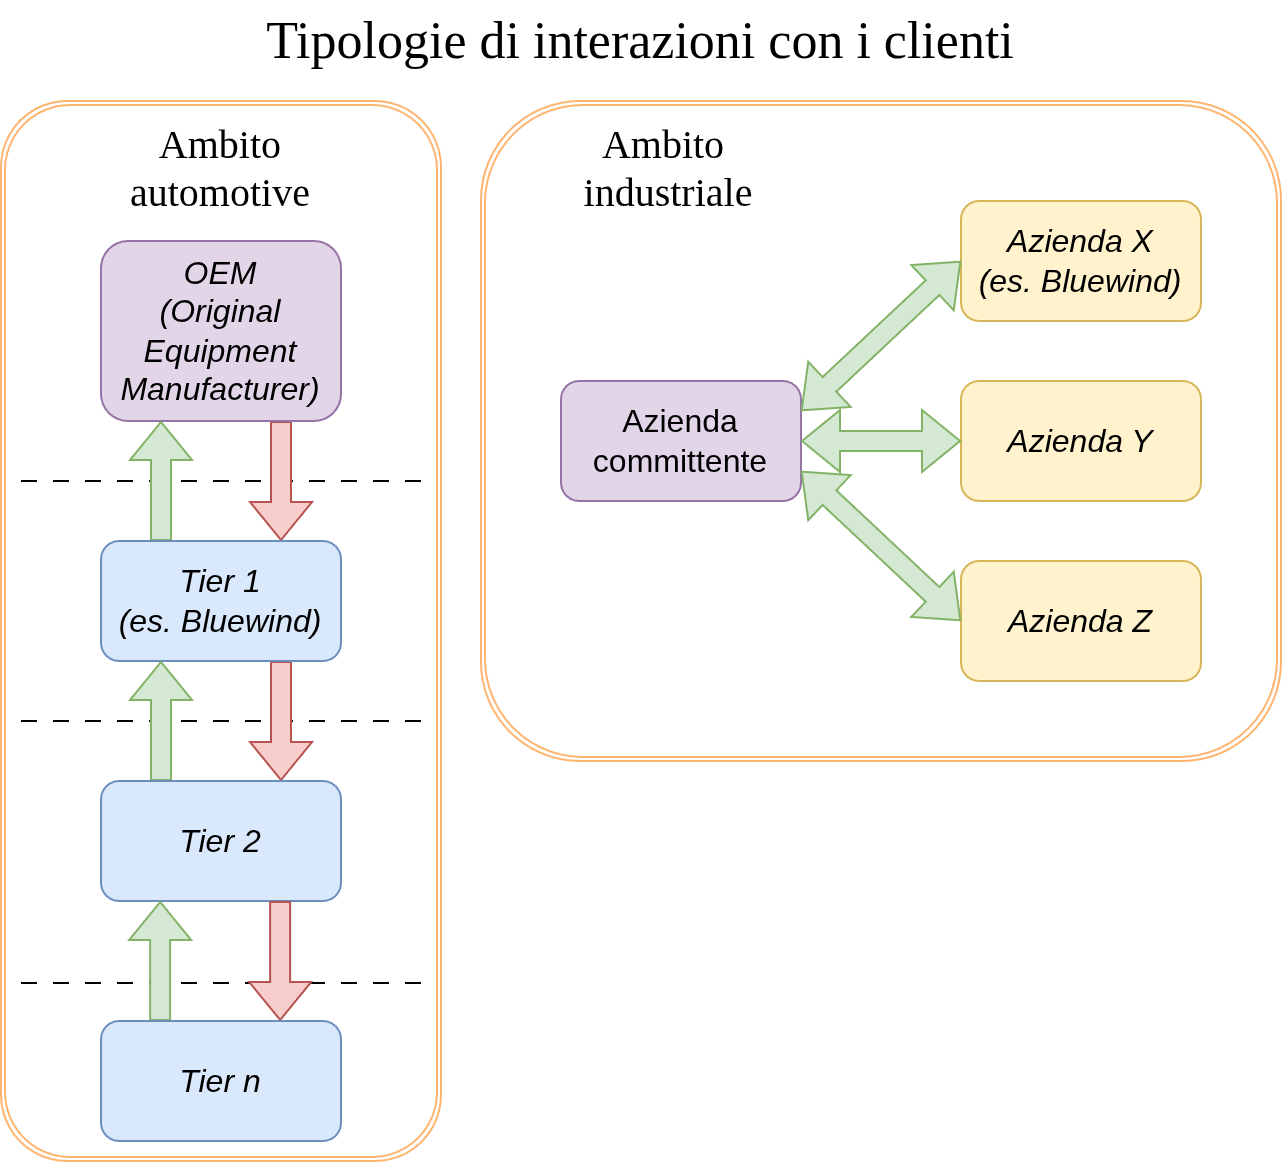
\includegraphics[width=\textwidth]{img/interazioni_clienti.png}}
    \caption{\centering Schema che rappresenta la differenza di interazioni tra i clienti in ambito \textit{automotive} e quelli in ambito industriale generale}
    \vspace{0.1cm}
    {\footnotesize Elaborazione originale dell'autore\par}
\end{figure}


\section{Lo \textit{stack} tecnologico aziendale}
\iffalse
In questa sezione parlo di quali sono le tecnologie utilizzate maggiormente all'interno dell'azienda sia in ambito di sviluppo che di processi organizzativi.
\fi
\noindent
Gli anni di attività hanno portato \textit{Bluewind} a prendere confidenza con diverse tecnologie e strumenti, che spaziano in vari casi di utilizzo.
La loro adozione tuttavia è fortemente influenzata dalle richieste del cliente.
Difatti, \textit{Bluewind} tende a non avere uno \textit{standard} fisso su quali strumenti utilizzare, e si rifà molto a quello che viene utilizzato dall'azienda cliente.
Questo avviene perché lavorando a stretto contatto con i propri clienti, e i rispettivi team di sviluppo, spesso su progetti già avviati, è necessario per \textit{Bluewind} allinearsi con il metodo di lavoro del cliente.
Spesso tale scelta è motivata anche dal fatto che il prodotto finale comprende anche il codice sorgente, il quale rimane al cliente che potrebbe volerci lavorare ulteriormente in futuro.\\\\
\noindent
Nonostante questa dinamica, vi sono delle tecnologie che a cui ricorrono con maggiore frequenza o alle quali, in mancanza di specifiche richieste, preferiscono affidarsi.

%sviluppo
\subsection{Il linguaggio \textit{C}}
\noindent
Il linguaggio \textit{C} rimane il linguaggio dominante nel settore \textit{embedded}, in quanto offre un controllo quasi diretto sull'\textit{hardware} (registri, memoria, interrupt) mantenendo comunque un livello di astrazione superiore all'\textit{Assembly}.
Su microcontrollori con risorse limitate (specialmente in termini di memoria, si parla anche pochi \textit{kilobyte} di \textit{RAM}) non c'è modo di adottare linguaggi più moderni con funzionalità più complesse come il \textit{garbage collector} o l'\textit{overhead}, occorre invece qualcosa che offrà prevedibilità nei tempi di esecuzione e controllo esplicito sull'allocazione.
Su questo tema il linguaggio \textit{C} rimane ancora oggi il punto di riferimento per il settore.
Va detto però che questo controllo è anche notoriamente il suo punto debole: niente \textit{memory safety} nativa, puntatori pericolosi, comportamenti \textit{undefined} sono rischi che negli ambiti \textit{safety-critical} (come quello \textit{automotive}, o medico) vanno trattati con assoluto riguardo.\\
Nel capitolo successivo parlerò più a fondo delle regole \gls{misra} che rappresentano un'importante \textit{standard} per limitare gli errori più comuni.


\subsection{Il linguaggio \textit{Assembly}}
\noindent
Seppur non accada con grande frequenza, il \textit{C} a volte non è sufficiente, e si rende necessaria l'adozione del linguaggio \textit{Assembly} per raggiungere il livello di controllo richiesto.
L'\textit{Assembly} resta il linguaggio più basso disponibile nell'\textit{embedded}, avendo una corrispondenza vicina all'uno a uno con le istruzioni macchina dell'architettura.
Quindi viene utilizzato quando serve controllo assoluto sull'\textit{hardware}, accesso a istruzioni specifiche non esposte dal \textit{C} o un'ottimizzazione estrema di alcune funzioni critiche.


\subsection{Strumenti proprietari di aziende \textit{partner} come \textit{Infineon} e \textit{ST}}
\noindent
Nell'ambito \textit{embedded} è spesso richiesto l'utilizzo di componenti \textit{hardware} costruite su misura per il loro caso di applicazione.
Ne consegue che, di progetto in progetto, ogni dispositivo per cui andrà sviluppato il \textit{software} sia leggermente diverso, per le componenti (connettori, microprocessori, adattatori ecc.) di cui è composto.
Per questo motivo, le aziende fornitrici di \textit{hardware} come \textit{Infineon Technologies} e \textit{STMicroelectronics} (da notare che questi sono i \textit{brand} che io ho avuto modo di conoscere nella mia, relativamente breve, esperienza, tuttavia lo stesso ragionamento si applica anche ad altri \textit{partner} aziendali) mettono a disposizione delle schede che racchiudono un insieme predefinito di componenti che possono essere presenti nei dispositivi finali.
In questo modo le azienda produttrici di \textit{software} possono utilizzare le singole componenti di loro interesse, senza avere ancora a disposizione i dispositivi \textit{hardware} definitivi.
Questo semplifica lo sviluppo, rendendo più semplice per i programmatori ottenere un \textit{feedback} sul funzionamento del codice.\\\\
\noindent
Oltre alle schede, le aziende produttrici mettono a disposizione un gran catalogo di risorse per agevolarne l'utilizzo e la scrittura del codice, quali documentazione dettagliata sui prodotti, \gls{IDE} specifici per il tipo di scheda e altri \textit{tools} di monitoraggio e \textit{debugging}.

\subsection{\textit{Gitlab}}
\noindent
\textit{GitLab} è una piattaforma che integra in un unico strumento la gestione del codice sorgente, il controllo di versione basato su \textit{Git}, l'integrazione e distribuzione continua (\gls{ci_cd}), e la gestione dei progetti.
Si distingue inoltre da altre piattaforme concorrenti per la presenza di una versione \textit{self-hosted}, rendendola particolarmente apprezzata da aziende con esigenze specifiche di sicurezza e controllo sui propri dati.\\\\
Come ci si può aspettare, \textit{Bluewind} adotta questo strumento integrandolo all'interno dei propri \textit{server}, e rendendolo un elemento centrale all'interno della sua organizzazione aziendale.
Questo strumento si integra molto bene con il metodo \textit{agile} adottato dall'azienda, permettendo di organizzare, suddividere e tenere traccia delle attività in maniera più organizzata e meticolosa.

\subsection{\textit{StrictDoc}}
\noindent
\textit{StrictoDoc} è uno strumento gratuito e \gls{open_source_g} utilizzato per la scrittura di documentazione.
Viene adottato specialmente per l'analisi dei requisiti in quanto permette di fare più facilmente riferimento tra i requisiti e al codice, di creare la matrice di tracciabilità e di esportare la documentazione in altri formati, anche quelli usati da \textit{tools} proprietari.
È uno strumento su cui \textit{Bluewind} sta puntando molto per via della sua semplicità di utilizzo e della possibilità, in quanto \textit{open source} di aggiunge funzionalità \textit{custom} in base alla propria esigenza.

\iffalse
\begin{figure}[H]
    \centering
    \makebox[\textwidth][c]{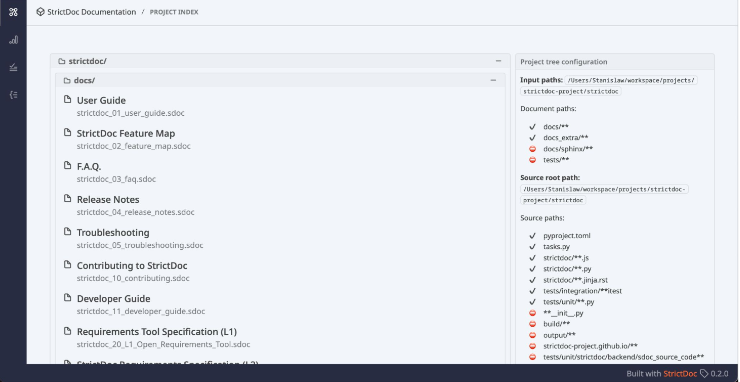
\includegraphics[width=\textwidth]{img/strictdoc_screen.png}}
    \caption{\centering Schermata del \textit{Project Index} di un progetto, preso dalla presentazione ufficiale di \textit{StrictDoc}}
    \vspace{0.1cm}
\end{figure}
\fi
%test
\subsection{\textit{PC-lint}}
\noindent
\textit{PC-lint} è uno strumento di analisi statica per \textit{C} e \textit{C++} utilizzato in ambienti \textit{safety-critical} per scoprire \textit{bug}, vulnerabilità e verificare il rispetto delle regole imposte dagli \textit{standard}, tra cui anche le regole \textit{MISRA}.\\
È uno strumento \gls{cli} e può essere integrato all'interno in un processo automatizzato di test e \textit{deployment}.

\subsection{Servizi e strumenti proprietari}
\noindent
Oltre ad affidarsi a tecnologie e strumenti esterni, \textit{Bluewind} ha una sua \textit{suite} di strumenti proprietari per la gestioni dei suoi processi interni.
Lo scopo principale è quello di offrire servizi che agevolino alcuni compiti : l'organizzazione tra il personale, controllare la disponibilità dei vari dipendenti, organizzare incontri, gestire lo \textit{smart working}, oppure, andando più sul tecnico, permettere di accedere da remoto a dispositivi \textit{hardware} condivisi tra più utenti e utili allo sviluppo.

\section{Propensione all'innovazione}
\iffalse
In questa sezione spiego come l'azienda si rivolge al tema dell'innovazione e quali metodi/processi segue per inseguire tale fine.
\fi
\noindent
In un periodo come quello attuale, in cui l'avanzamento tecnologico lascia poco spazio all'indecisione, avere una chiara idea e un chiaro metodo di approccio all'innovazione è fondamentale per potersi posizionare correttamente all'interno del mercato e per poter impiegare al meglio tempo e risorse.
Per questo motivo all'interno di \textit{Bluewind} è presente un impegno molto sentito verso il tema dell'innovazione che e coinvolge tutto il personale.\\\\
Il loro specifico mercato di riferimento tuttavia non li aiuta: lavorare in settori dove la sicurezza e la prevedibilità dei sistemi sono aspetti profondamente critici, porta le aziende a dover avanzare con cautela nell'esplorare nuove opportunità.
Un ostacolo concreto sono i vincoli posti dai requisiti obbligatori a cui le aziende devono sottostare.\\
Un chiaro esempio di queste limitazioni è l'adozione dell'IA: l'utilizzo dei algoritmi di \gls{ml_g} è ancora un argomento non del tutto esplorato vista la mancanza di regolamentazione a riguardo, ma soprattutto perché aggiunge una variabile imprevedibile all'interno di un contesto che spesso non se la può permettere.\\
Nonostante ciò ci sono stati dei passi avanti da parte dell'azienda anche su questo tema, e persiste il desiderio di approfondire anche questa tematica.\\\\
In generale, \textit{Bluewind} segue un approccio molto attivo sul tema dell'innovazione, difatti ho notato in molti dipendenti la predisposizione ad accogliere le novità e a interessarsi fin da subito a come trarne vantaggio.
Oltre a ciò l'azienda intraprende costantemente iniziative volte al miglioramento dei propri processi interni, sia tramite collaboratori esterni, sia con ricerche svolte dai dipendenti stessi.\\
Una parte importante in questo piano sono i tirocini studenteschi, i quali permettono a \textit{Bluewind} di esplorare nuove tematiche e soluzioni per le quali altrimenti non ci sarebbero il tempo o le risorse da dedicare.
